\chapter{Random Variables}
\label{fundamentals}

In this Chapter some basic concepts, that will be used throughout the remaining part of this notes, are reviewed.

\section{Random Variable}
\label{random-variables}

In probability and statistics a random variable is described as a variable whose values depend on outcomes of a random phenomenon. 
%<<<<<<< HEAD
%=======
%<<<<<<< HEAD:financial_markets_lectures/random_variables2.tex
%It can be formalized as a certain function that is defined over the set of all possible outcomes, referred to as sample space $\Omega$. 
%
%For example, in the event of a coin toss, only two outcomes are possible: heads or tails. If instead the random variable is designated to represent the sum of the resulting numbers after three dice are rolled, it could be 3 ($1 + 1+ 1$), 18 ($6 + 6 + 6$), or somewhere in between.
%
%In the corporate world, random variables can be assigned to properties such as the average price of an asset over a given time period, the return on investment after a specified number of years, the estimated turnover rate at a company within the following six months, etc. Risk analysts assign random variables to risk models when they want to estimate the probability of an adverse event occurring. 
%
%Since in all cases that are taken into account here, $X$ is real-valued, formally a random variable can be understood as a measurable function defined on a probability space that maps from the sample space to the real numbers.
%=======
%>>>>>>> a1ac7f24ce4566e11029c1fa992020cf704cc565

The word "variable" in random variable is a misnomer since it is actually a function. And like all well behaved functions, a random variable, say $X$, has a domain and a range.

The domain $\Omega$ of $X$ is the sample space of random outcomes. These outcomes arise when some stochastic experiment is performed. The outcomes may or may not be numeric. 

For example, in the event of a coin toss, only two outcomes are possible: heads or tails. If instead the random variable is designated to represent the sum of the resulting numbers after three dice are rolled, it could be 3 ($1 + 1+ 1$), 18 ($6 + 6 + 6$), or somewhere in between.

In the corporate world, random variables can be assigned to properties such as the average price of an asset over a given time period, the return on investment after a specified number of years, the estimated turnover rate at a company within the following six months, etc. Risk analysts assign random variables to risk models when they want to estimate the probability of an adverse event occurring. 

%It can be formalized as a certain function that is defined over the set of all possible outcomes, referred to as sample space $\Omega$. 

Since in all cases that are taken into account here, $X$ is real-valued, formally a random variable can be understood as a measurable function defined on a probability space that maps from the sample space to the real numbers, i.e. the range.
%<<<<<<< HEAD
%=======
%>>>>>>> a1ac7f24ce4566e11029c1fa992020cf704cc565:financial_markets_lectures/random_variables.tex
%>>>>>>> a1ac7f24ce4566e11029c1fa992020cf704cc565
%
%\begin{equation}
%X:\Omega \rightarrow E
%\end{equation}
%where $E=\mathbb {R}$, or in words, $E$ represents the set of real numbers. 
%<<<<<<< HEAD
%=======
%<<<<<<< HEAD:financial_markets_lectures/random_variables2.tex

Random variable's values might represent the possible outcomes of a yet-to-be-performed experiment. They may also conceptually represent either the results of an "objectively" random process (such as rolling a die). As a function, a random variable is required to be measurable, which allows for probabilities to be assigned to its potential values. 

A random variable is different from an algebraic one. An equation variable is an unknown value that can be calculated. The equation $10 + x = 13$ shows that we can calculate the specific value for $x$ which is 3. On the other hand, a random variable has a set of values, and any of those values could be the resulting outcome.

When the range of possible values for $X$ is un-countably infinite then $X$ is called a \emph{continuous random variable} and its distribution can be described by a \emph{probability density function} (PDF). Contrary if the range is countable, the random variable is called a \emph{discrete random variable} and its distribution can be interpreted as a discrete probability distribution.

The PDF is used to specify the probability of the random variable falling within a particular range of values. By definition 
the probability density function is non-negative everywhere, and its integral over the entire space is equal to 1.
Left plot in Fig.~\ref{fig:pdf_pmf} shows an example of Gaussian probability density function.

%=======
%>>>>>>> a1ac7f24ce4566e11029c1fa992020cf704cc565

Why then is $X$ called a random variable? It’s because $X$ outputs values using a probability distribution that is supposed to represent the likelihoods of occurrences of events in the sample space. 

%A random variable is different from an algebraic one. An equation variable is an unknown value that can be calculated. The equation $10 + x = 13$ shows that we can calculate the specific value for $x$ which is 3. On the other hand, a random variable has a set of values, and any of those values could be the resulting outcome.

When the range of possible values for $X$ is un-countably infinite then $X$ is called a \emph{continuous random variable} and its distribution can be described by a \emph{probability density function} (PDF). Contrary if the range is countable, the random variable is called a \emph{discrete random variable} and its distribution can be interpreted as a discrete probability distribution.

The PDF is used to specify the probability of the random variable falling within a particular range of values. By definition 
the probability density function is non-negative everywhere, and its integral over the entire space is equal to 1.
Left plot in Fig.~\ref{fig:pdf_pmf} shows an example of Gaussian probability density function.

%<<<<<<< HEAD
%=======
%>>>>>>> a1ac7f24ce4566e11029c1fa992020cf704cc565:financial_markets_lectures/random_variables.tex
%>>>>>>> a1ac7f24ce4566e11029c1fa992020cf704cc565
In the context of discrete random variables the probability density function is usually referred to as \emph{probability mass function} (PMF). Right plot in Fig.~\ref{fig:pdf_pmf} shows an example of discrete probability density function.

\begin{figure}[htb]
	\centering
	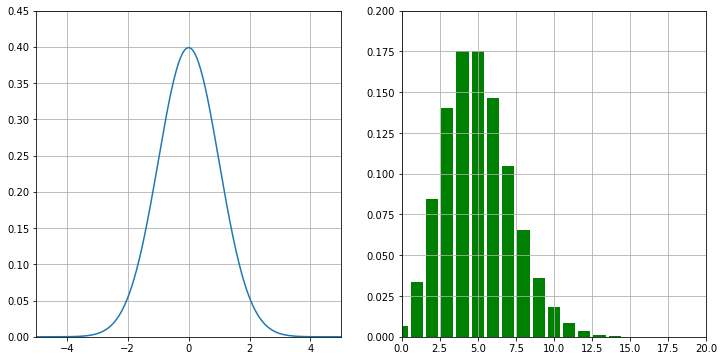
\includegraphics[width=1.\textwidth]{figures/pdf_pmf.png}
	\caption{On the left an example of continuous probability density function (Normal), on the right a discrete probability mass function (Poissonian).}
	\label{fig:pdf_pmf}
\end{figure}

\subsection{Cumulative Distribution and Quantile Functions}
\label{sec:quantile-function}

The \emph{cumulative distribution function} (CDF) $F$ of a random variable $X$, evaluated at $x$, gives the probability that $X$ will take a value less than or equal to $x$

\begin{equation}
F_X(x) = P(X \le x)\qquad\mathrm{or~equivalently}~\int_{-\infty}^{x}{f(X)dX}
\end{equation}
so it gives the area under the probability density function $f$ from minus infinity to $x$.
The probability that $X$ lies in the interval $(a,b]$ is therefore

\begin{equation}
P(a> X \le b)=F_{X}(b)-F_{X}(a)\qquad\mathrm{or}~\int_a^b{f(X)dX}
\end{equation}
Notice that by the previous definition any random variable can be conveniently described by its cumulative distribution too.

The \emph{quantile function} $Q$, associated with a probability distribution of a random variable, specifies the value $x$ of the random variable such that the probability $p$ of the variable being less than or equal to that value equals the given probability. It is also called the percent-point function (PPF) or inverse cumulative distribution.

In terms of the cumulative distribution function $F$, the quantile function $Q$ returns the value $x_p$ such that 

\begin{equation}
F_{X}(x_p)=P(X\le x_p)=p
\end{equation}
So the quantile function can be considered the "inverse" of the cumulative distribution function: given a probability $p$ (or a value of the CDF) it returns the $x$ at which the CDF reaches this probability, so we can write $Q=F^{-1}$.

In Fig.~\ref{fig:percentile} an example related to the Gaussian distribution is shown. On the left side the Gaussian PDF is drawn, the red area represents the 30\% of the total area (which is 1 by definition). On the right the corresponding CDF is plotted, the point at which the CDF reaches 30\% is highlighted. The corresponding quantile value is also indicated and is $-0.5244$.

\begin{figure}[htb]
	\centering
	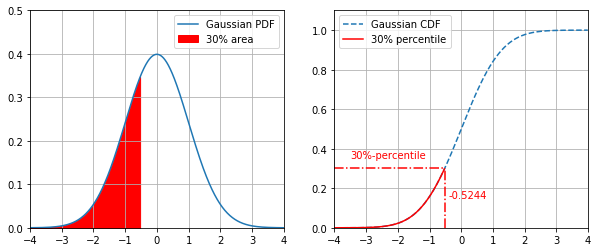
\includegraphics[width=1.\textwidth]{figures/percentile.png}
	\caption{On the left a standard normal distribution, the filled region represent the 30\% of the total area under the curve. On the right the corresponding CDF with the 30\% point and the relative quantile highlighted.}
	\label{fig:percentile}
\end{figure}

The computation of CDF and quantiles is quite simple in \texttt{python}. The implementation of many distributions is available in \texttt{scipy.stats} module and for each of them the methods \texttt{cdf(x)} and \texttt{ppf(x)} can be used to evaluate CDF and quantile respectively.

\begin{ipython}
from scipy.stats import norm

quantile = norm.ppf(0.3)
cdf = norm.cdf(quantile)
print ("30%-quantile of standard normal is {}".format(quantile))
print ("CDF value at {}: {}".format(quantile, cdf))
\end{ipython}
\begin{ioutput}
30%-quantile of standard normal is -0.5244005127080409
CDF value at -0.5244005127080409: 0.29999999999999993
\end{ioutput}

If instead of a distribution a dataset is involved, the quantile can be determined using the function \texttt{numpy.percentile} (e.g. this will be useful when estimating VaR). Notice that in this case we are talking about \emph{percentile} which is the \emph{quantile} times 100 (e.g. 50-percentile is equivalent to 0.5-quantile).

\begin{ipython}
import numpy
dist = [1, 2, 3, 4, 5, 6, 7, 8, 9]

# first argument the data-set
# second argument a list of percentiles
perc = numpy.percentile(dist, [1, 50])
print (perc)
\end{ipython}
\begin{ioutput}
[1.08 5.  ]
\end{ioutput}

\subsection{Expected Value}\label{sec:expected-value}

Since a random variable is connected to a probabilistic event, it is necessary to take into account all the possible values it can take for its evaluation. This is done with the \emph{expected value}
which is a generalization of the weighted average, and is intuitively the arithmetic mean of all the possible realizations of a random variable \(X\).

\subsubsection{Discrete Case}
Consider a random variable with a finite number of outcomes $(x_{1},x_{2},\ldots ,x_{k})$ occurring with probabilities $(p_{1},p_{2},\ldots ,p_{k})$ respectively. The expectation of $X$ is then defined as

\begin{equation}
	\mathbb{E}[X]=\sum _{i=1}^{k}x_{i}\,p_{i}=x_{1}p_{1}+x_{2}p_{2}+\cdots +x_{k}p_{k}
\end{equation}

Since $p_{1}+p_{2}+\cdots +p_{k}=1$, the expected value is the average of the $x_{i}$ weighted by their probabilities $p_{i}$.

%By definition, the expected value of a constant random variable \(X=c\) equals its constant value \(c\). Instead the expected value of a random variable \(X\) with equiprobable outcomes \((c_{1},\ldots ,c_{n})\) is defined as the arithmetic mean of the terms \(c_i\). 

As an example let $X$ represent the outcome of a single roll of a fair six-sided die. The possible values for $X$ are 1, 2, 3, 4, 5, and 6, all of which are equally likely with probability $1/6$.

The expectation of $X$ is then

\begin{equation*}
	\mathbb{E}[X]=1\cdot {\frac {1}{6}}+2\cdot {\frac {1}{6}}+3\cdot {\frac {1}{6}}+4\cdot {\frac {1}{6}}+5\cdot {\frac {1}{6}}+6\cdot {\frac {1}{6}}=3.5
\end{equation*}
If one rolls the die $n$ times and computes the results average, then as $n$ grows, this average converges to the expected value.

\subsubsection{Continuous Case}
If $X$ is a random variable with a probability density function, $f(x)$, then the expected value is defined as

\begin{equation}
\mathbb{E}[X]=\int_{\Omega}xf(x)dx
\end{equation}
For multidimensional random variables, the expected value is defined per component, that is,

\begin{equation}
\mathbb{E}[(X_{1},\ldots ,X_{n})]=(\mathbb{E} [X_{1}],\ldots ,\mathbb{E}[X_{n}])
\end{equation}

\subsection{Some Properties of Expected Value}
\label{some-properties}

\begin{itemize}
\tightlist
\item Let $\mathbb{1}_{A}$ denote the indicator function of an event $A$ (i.e. a function whose value is 1 if the event $A$ happens, 0 otherwise), then

\begin{equation}
\mathbb{E}[\mathbb{1}_{A}] = 1\cdot P(A)+0\cdot P(\Omega \setminus A)= P(A)
\end{equation}

\item the expected value operator \(\mathbb{E}\) is linear in the sense that, for any random variables $X$ and $Y$, and a constant $a$
\begin{equation}
\begin{cases}
\mathbb{E}[X+Y] = \mathbb{E}[X] + \mathbb{E}[Y] \\
\mathbb{E}[aX] = a\mathbb{E}[X]
\end{cases}
\end{equation}

This means that the expected value of the sum of any finite number of random variables is the sum of the expected values of the individual random variables, and the expected value scales linearly with a multiplicative constant;

\item the expected value of a measurable function of $X$, $g(X)$, given that $X$ has a probability density function $f(x)$, is given by 

\begin{equation}
\mathbb{E}[g(X)] = \int_{\Omega}g(x)f(x) dx
\end{equation}

This formula also holds in multidimensional case, when $g$ is a function of several random variables, and $f$ is their joint density;

\item $n$ random variables $X_1 ,\ldots , X_n$ are independent if the following property holds for all positive functions $f_1 ,\ldots , f_n$

\begin{equation}
\mathbb{E}[f_1 (X_1 )\cdots f_n (X_n )] = \mathbb{E}[f_1 ( X_1 )] \cdots \mathbb{E}[f_n (X_n )]
\end{equation}
\end{itemize}


%
%We have seen so far how to generate a sequence of random numbers from U
%{[}0, 1{]}. However, most of the simulations include the sampling of
%random variables, or even random vectors in a mul- tidimensional case,
%from specified, not uniform distributions. Sampling of nonuniform random
%variates is done indirectly, i.e.~one transforms samples from the
%uniform to a desired nonuniform distribution. Accordingly, each
%realization of a nonuniform random variable is directly obtained from a
%single uniform variate or from a sequence of uniforms {[}46, p.54{]}.
%There are numerous algorithms that allow you to generate random numbers
%from a certain desired distribution. However, two main criteria in order
%to choose between them are accuracy and speed.


%
%\hypertarget{correlated-normal-variables-and-vectors}{%
%\subsubsection{Correlated normal variables and
%	vectors}\label{correlated-normal-variables-and-vectors}}
%
%A \(d\)-variate normal distribution \(\phi(\mu, \Sigma)\) is generally
%specified by its mean vector \(\mu\) and variance- covariance matrix
%\(\Sigma\). Random vectors from a multivariate normal distribution can
%be generated directly by generating a \(d\)-vector of iid standard
%normal deviates \(z' = (z_1 , z_2 ,\dots , z_d)\).
%
%Next we know from the linear transformation property that if the vector
%\(z∼\phi_d (0,I)\) and \(x = \mu + Az\), then \(x ∼\phi_d (\mu, AA')\).
%Therefore, we can generate a sequence of univariate normal random
%variables \(z_i\) and put them into a vector \(z\). Thus the challenge
%is merely made up of finding the matrix \(A\) for which the property
%\(AA' = \Sigma\) holds. The representation of \(\Sigma\) as \(AA'\) with
%\(A\) as a lower triangular matrix is denoted as a Cholesky
%factorization of the variance-covariance matrix \(\Sigma\). If
%\(\Sigma\) is symmetric positive definite there is a Cholesky
%factorization and the sampling of multivariate normals is easily done by
%basically sampling from a univariate \(\phi(0,1)\).
%
%In some applications in finance random variables or vectors are required
%to depend on each other in a prescribed way, i.e.~they must not be
%totally uncorrelated. Correlated random variables are calculated
%according to the following algorithm:
%
%\begin{enumerate}
%\def\labelenumi{\arabic{enumi}.}
%\tightlist
%\item
%calculate the Cholesky factorization \(AA′ = \Sigma\),
%\item
%calculate \(z ∼ \phi(0,I)\) by component, for \(i = 1,2,\ldots ,d\),
%\item
%\(x=\mu + Az\), then \(x∼\phi (\mu, \Sigma )\).
%\end{enumerate}
%
%Suppose we have a two-dimensional case, \(d = 2\). Next we are looking
%for a vector \(x' = (x_1 , x_2 ) ∼ \phi (0, \Sigma )\). The correlation
%between \(x_1\) and \(x_2\) is denoted by \(\rho\) and thus the Cholesky
%factorization provides \(\Sigma = AA'\)
%
%\[\begin{bmatrix}
%\sigma_1^2 & \rho\sigma_1 \sigma_2\\
%\rho\sigma_1 \sigma_2 & \sigma_2^2 
%\end{bmatrix} = 
%\begin{bmatrix}
%\sigma_1 & 0\\
%\rho\sigma_2 & \sigma_2\sqrt{1-\rho^2} 
%\end{bmatrix}
%\begin{bmatrix}
%\sigma_1 & \rho\sigma_2 \\
%0 & \sigma_2\sqrt{1-\rho^2} 
%\end{bmatrix}\]
%
%If \(z_1\) and \(z_2\) are independent and from \(\phi(0, 1)\), then
%
%\[\begin{bmatrix}
%x_1\\
%x_2 
%\end{bmatrix} = A
%\begin{bmatrix}
%z_1\\
%z_2 
%\end{bmatrix} = 
%\begin{bmatrix}
%\sigma_1 z_1\\
%\sigma_2 (\rho z_1 + \sqrt{1-\rho^2}z_2) 
%\end{bmatrix}
%\]
%
%are distributed according to \(\phi(0, \Sigma)\).
%
%\begin{codebox}
%\prompt{In}{incolor}{ }{\boxspacing}
%\begin{Verbatim}[commandchars=\\\{\}]
%	
%\end{Verbatim}
%\end{codebox}

\section*{Exercises}
\begin{question}
A random variable $X$ that assumes values in the interval $[0, 1]$ has density function $f(x) = a + b x$,
where $a$ and $b$ are two constants to be determined.

\begin{enumerate}[label={\emph{\alph*})}]
\tightlist
\item Compute $a$ and $b$ such that $f(x)$ has a PDF with probability density in $X = 1$ being the double of the probability density in $X = 0$;
\item compute the quartiles (0.25, 0.5, 0.75 quantiles) of the random variable $X$.
\end{enumerate}
\end{question}

\begin{solution}
\begin{enumerate}[label={\emph{\alph*})}]
\tightlist
\item Given the PDF of the random variable $f(x) = a + bx$ the two constants $a$ and $b$ can be determined by imposing the normalization of the density function and the required conditions at the boundaries:

\begin{equation*}
\begin{cases}
f(1) = 2\cdot f(0)\\
\int_0^1 f(x)dx = 1
\end{cases}  
\end{equation*}
The first equation gives $a+b = 2a \implies a = b$ while the integral can be easily solved

\begin{equation*}
\int_0^1 f(x)dx = \left(ax + \frac{a}{2}x^2\right|^1_0 = 1 \implies a = \frac{2}{3}
\end{equation*}

\item From the first point we fully determined the PDF $f(x) = \frac{2}{3}(1 + x)$. To compute the quartiles it is first necessary to integrate it to get the corresponding CDF 
\begin{equation*}
F(x) = \int_0^{1/4} f(x)dx = \frac{2}{3}\left(x + \frac{1}{2}x^2\right) = \frac{1}{3}x^2 + \frac{2}{3} x  - \frac{1}{4}
\end{equation*}

Then the first quartile ($Q_1$) is given by $F^{-1}(x) = 1/4$ and similarly for the others
\begin{gather*}
\frac{1}{3}x^2 + \frac{2}{3} x  = \frac{1}{4} \\
Q_1 = -1 \pm \frac{3}{2}\sqrt{\frac{7}{9}} = \frac{1}{2}(\sqrt{7} - 2) = 0.3229\\
Q_2 = \dots = 0.5811\\
Q_3 = \dots = 0.8028
\end{gather*}
\end{enumerate}
\end{solution}

\begin{question}
\label{ex:greedy_pig}
The Greedy Pig Game is a simple dice game. It is played with one single die and the goal is to reach 100 points. Each player in turn starts to roll the die, if it results to be in [2, 6] the corresponding points are acquired and the player can decide either to continue to roll or to stop. If a 1 is rolled the player scores a 0 and her turn ends.

\begin{itemize}
\item What is the expected number of points for one roll ?
\item Imagine a player that has collected $k$ points. Compute and draw the expected points obtained with a further roll. What can be concluded from this plot ?
\end{itemize}
\end{question}

\cprotEnv\begin{solution}
The expected number of points for one roll is the weighted average of the possible points [2, 6] (when the die is 1 no points are assigned) with the probability of 1/6.
\begin{ipython}
ex_roll = 0
for i in range(2, 7):
    ex_roll += 1/6*i

print (ex_roll)
\end{ipython}
\begin{ioutput}
3.3333333333333
\end{ioutput}

If the current points of a player are $k$, in computing the expectation, beside the [2, 6]*1/6 terms, it has to be added a $-k\cdot 1/6$ term in case a 1 is rolled (i.e. in this case the total score goes to 0 and the turn ends).
\begin{ipython}
from matplotlib import pyplot as plt

exps = []
for k in range(1, 51):
    exp = -k*1/6
    for i in range(2, 7):
        exp += 1/6*i
    exps.append(exp)

fig = plt.figure(figsize=(10,8))
plt.plot(range(1, 51), exps)
plt.grid(True)
plt.xlabel("current turn points ($k$)")
plt.ylabel("expected points next roll")
plt.show()
\end{ipython}

Figure~\ref{fig:greedy_pig_expec} shows the expected points distribution in the next roll as a function of the current player points. It looks like that when the player has more than 20 points the expectation becomes negative, so it is not anymore convenient to keep rolling. This is a fundamental clue to derive a game strategy: \emph{keeps rolling until you reach 20 points}.

\begin{figure}[htbp]
	\begin{center}
		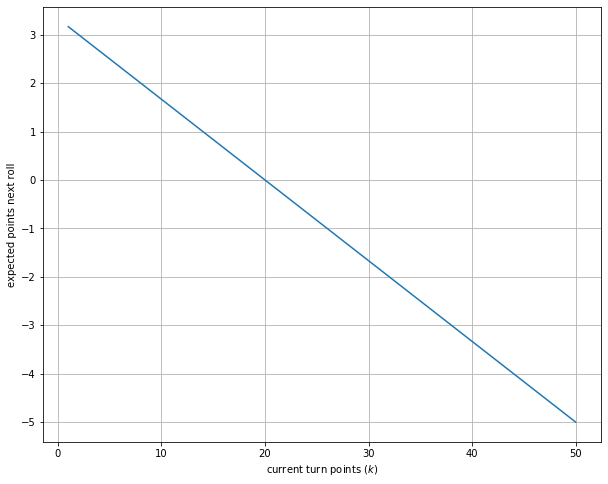
\includegraphics[width=0.7\linewidth]{figures/greedy_pig_expectation}
	\end{center}
\caption{Expected points in the next roll as a function of the current turn points.}
\label{fig:greedy_pig_expec}
\end{figure}
\end{solution}

\begin{question}
Let $X$ be a random variable with density function

\begin{equation*}
f(x) = 
\begin{cases}
k(1 - x^2),~\textrm{if}~0 \leq x \leq 1\\
0,~\textrm{otherwise}		
\end{cases}
\end{equation*}
Find $k$, together with the expectation and the variance of the random variable $Y$ defined as $Y = 3X - 1$.
\end{question}

\cprotEnv\begin{solution}
\label{ex:variance}
To find the value of $k$ we can exploit the normalization condition for a probability density:

\begin{equation*}
\begin{gathered}
\int_\Omega f(x) d\Omega = 1\\
\int_{0}^{1}k(1-x^{2})dx = k\left(x-\frac{1}{3}x^{3}\right|_{0}^{1}= k\left(1-\frac{1}{3}\right) \\
k\left(1-\frac{1}{3}\right) = 1 \implies k = \frac{3}{2}
\end{gathered}
\end{equation*}

The expectation of the variable $Y$ instead equals to
\begin{equation*}
\mathbb{E}[Y] = 3\mathbb{E}[X] - 1
\end{equation*}	
So
\begin{equation*}
\begin{gathered}
\mathbb{E}[X] = \frac{3}{2}\int_{0}^{1}x(1-x^2)dx = \frac{3}{2}\left(\frac{1}{2}x^2-\frac{1}{4}x^{4}\right|_{0}^{1} = \frac{3}{2}\left(\frac{1}{2}-\frac{1}{4}\right) = \frac{3}{8} \\
\mathbb{E}[Y] = 3\cdot\frac{3}{8} - 1 = \frac{1}{8} 
\end{gathered}
\end{equation*}
And finally for the variance:
\begin{equation*}
\begin{aligned}
Var[Y] = & \mathbb{E}[Y^2] - (\mathbb{E}[Y])^2 = \frac{3}{2}\int_{0}^{1}(9x^2 - 6x + 1)(1-x^2)dx - \frac{1}{64} = \\  &\frac{3}{2}\int_{0}^{1}(- 9x^4 + 6x^3 + 8x^2 - 6x + 1)dx - \frac{1}{64} = 
\frac{3}{2}\left(- \frac{9}{5}x^5 + \frac{6}{4}x^4 + \frac{8}{3}x^3 - 3x^2 + x\right|_{0}^{1} - \frac{1}{64} = \\
& \frac{3}{2}\left(- \frac{9}{5} + \frac{6}{4} + \frac{8}{3} - 3 + 1\right) - \frac{1}{64} = \frac{11}{20} - \frac{1}{64} = \frac{171}{320}
\end{aligned}
\end{equation*}

Alternatively it can be demonstrated that the variance of a random variable $Y = a + bX$ can be computed as $Var[Y] = b^2 Var[X]$. Indeed starting from the general form of the variance $Var[Y] = \mathbb{E}[Y^2] - (\mathbb{E}[Y])^2$ and computing each term of the right hand side of the equation 

\begin{equation}
\begin{gathered}
\mathbb{E}[Y^2] = \mathbb{E}[(a+bX)^2] = \mathbb{E}[b^2X^2 + 2abX + a^2] = b^2\mathbb{E}[X^2] + 2ab\mathbb{E}[X]+ a^2  \\
\mathbb{E}[Y]^2 =  (b\mathbb{E}[X] + a)^2 = b^2\mathbb{E}[X]^2 + 2ab\mathbb{E}[X]+ a^2  
\label{eq:each_var}
\end{gathered}
\end{equation}
Substituting Eqs.~\ref{eq:each_var} into the general form of the variance 
\begin{equation}
\begin{gathered}
Var[Y] = b^2\mathbb{E}[X^2] + 2ab\mathbb{E}[X]+ a^2 - (b^2\mathbb{E}[X]^2 + 2ab\mathbb{E}[X]+ a^2) \\ 
= b^2\mathbb{E}[X^2] - b^2\mathbb{E}[X]^2 = b^2 Var[X]
\end{gathered}     
\end{equation}

So $Var[Y] = 9\mathbb{E}[X]$.
\end{solution}

\begin{question}
We want to insure a car of 12000 EUR. The probability that a car is involved in an accident during a year is 0.15 in which case the amount of damage is

\begin{itemize}
\tightlist
\item 20\% of its value with probability 0.8;
\item 60\% of its value with probability 0.12;
\item 100\% of its value with probability 0.08.
\end{itemize}
Find the first annual premium the insurer must charge to have the expected cost of the company equal to 0.
\end{question}

\cprotEnv\begin{solution}
\begin{ipython}
print (f"{0.15 * 12000 * (0.8*0.2 + 0.6*0.12 + 0.08):.2f} EUR")
\end{ipython}
\begin{ioutput}
561.60 EUR
\end{ioutput}
\end{solution}

\begin{question}
The daily expenditure ($X$, in euros) spent by a certain customer in a department store is distributed according to the following density function:

\begin{equation*}
f(x) = 
\begin{cases}
x^2/9000,~\textrm{if}~0 \leq x \leq 30\\
0,~\textrm{otherwise}		
\end{cases}
\end{equation*}

\begin{enumerate}[label={\emph{\alph*})}]
\item calculate the probability that the client has a daily spending between 15 and 20 EUR;
\item what is his/her expected daily expenditure ?;
\item next winter the department store is granting the following "discount vouchers", whose amount depends on the client's expenditure: 1 EUR for spending between 10 and 20 EUR, 1.5 EUR for spending between 20 and 25 EUR,
3 EUR if the expense exceeds 25 EUR. Derive the distribution and the expected value of the discounts obtained by the client.
\item the customer has paid for his/her purchases in the store with a credit card which applies a 4\% charge. What is the probability that the customer has paid (with charges included) between 10 and 15 EUR ?
\end{enumerate}
\end{question}

\cprotEnv\begin{solution}
\begin{enumerate}[label={\emph{\alph*})}]
\tightlist
\item First we need to calculate the CDF by simple integration of the given PDF.
\begin{ipython}
def F(x):
    return x**3/27000

P = F(20) - F(15)
print (P)
\end{ipython}
\begin{ioutput}
0.17129629629629628
\end{ioutput}
\item The expected expense is given by $\int_{0}^{30} xf(x) dx = x^4/36000$
\begin{ipython}
def tot(x):
    return x**4/36000

print (tot(30))
\end{ipython}
\begin{ioutput}
22.5	
\end{ioutput}

\item The expected discount value is given by the weighted average of each discount times the probability of spending the corresponding amount of money:
\begin{ipython}
expected = 1 * (F(20)-F(10)) + 1.5 * (F(25) - F(20)) + 3 * (F(30) - F(25))
print (expected)
\end{ipython}
\begin{ioutput}
1.9467592592592593
\end{ioutput}

\item If the customer spent between 10 and 15 EUR with an extra charge of 4\% (by the usage of the credit card) the real expense limits has to be scaled by $1 - 0.04$, then the corresponding probability can be found using the function \texttt{F}:
\begin{ipython}
xmin = 10*0.96
xmax = 15*0.96
P = F(xmax) - F(xmin)

print (P)
\end{ipython}
\begin{ioutput}
0.07782399999999998
\end{ioutput}
\end{enumerate}
\end{solution}

\cprotEnv\begin{question}
An economist wishes to estimate the total cost of a project. His salary is composed of a fixed part of 12000 EUR plus a variable part of 300 EUR per day of work. The project can be performed between 7 and 11 days, and the economist has derived the following subjective probability distribution for the random variable $X$ (number of days it will take to implement the project):
\begin{ipython}
P = {7:0.10, 8:0.20, 9:?, 10:0.30, 11:0.10}
\end{ipython}
\begin{enumerate}[label={\emph{\alph*})}]
\tightlist
\item What is the probability that the project is carried out in 9 days? Justify your answer.
\item Determine the expected cost of the project and its variance. 
\end{enumerate}
\end{question}

\cprotEnv\begin{solution}
\begin{enumerate}[label={\emph{\alph*})}]
\tightlist
\item Since the assumption is that the work can be completed in between 7 and 11 days, the sum of $P$s has to equal 1. So $P(9)$ can be determined as
\begin{ipython}
P = {7:0.10, 8:0.20, 10:0.30, 11:0.10}
P[9] = 1 - (P[7]+P[8]+P[9]+P[10]+P[11])

print (f"{P[9]:.2f}")
\end{ipython}
\begin{ioutput}
0.30
\end{ioutput}
\item The expected cost of the project results
\begin{ipython}
expected_days = sum([d*p for d, k in P.items()])
E_C = 12000 + 300*expected_days

print (E_C)
\end{ipython}
\begin{ioutput}
14730.0	
\end{ioutput}

Remembering Solution~\ref{ex:variance} the variance in the costs $Var[C]$ (which follows a linear relationship with the number of days $C = 12000 + 300\cdot d$) becomes
\begin{ipython}
var_days = sum([(d**2)*p for d, k in P.items()])
b = 300
print (b**2 * var_days)
\end{ipython}
\begin{ioutput}
116100.0	
\end{ioutput}
\end{enumerate}
\end{solution}

\begin{question}
A casino advertises that the expected prize won by its clients is 600 EUR, with risk $\sigma$ = 360.
\begin{enumerate}[label={\emph{\alph*})}]
\tightlist
\item Calculate the probability that a player wins between 150 and 1050 EUR.
\item How would the above probability change if $\sigma$ = 420 ?
\item What is the probability that the prize won by a player deviates at least 504 EUR from its expectation?
\end{enumerate}
\end{question}

\cprotEnv\begin{solution}
In this case it is safe to assume that the wins are distributed as a Gaussian with mean 600 EUR and standard deviation 360 EUR. 
\begin{enumerate}[label={\emph{\alph*})}]
\tightlist
\item It is much easier to convert the initial distribution to a standard normal (zero mean and unit variance) using the following transformation
\begin{equation*}
x' = \frac{(x - \mu)}{\sigma}
\end{equation*}
in such a way \texttt{scipy.stats.norm} can be used.

\begin{ipython}
from scipy.stats import norm

# convert the two limits in the standard normal
xmin = (150 - 600)/360
xmax = (1050 - 600)/360

print (xmin, xmax)
print (norm.cdf(xmax) - norm.cdf(xmin))
\end{ipython}
\begin{ioutput}
-1.25 1.25
0.7887004526662893
\end{ioutput}

\item If the risk (i.e. uncertainty) increases the probability of winning an amount of money in the same range is expected to decrease. Let's check using the same technique as in the previous answer.
\begin{ipython}
xmin = (150 - 600)/420
xmax = (1050 - 600)/420

print (xmin, xmax)
print (norm.cdf(xmax) - norm.cdf(xmin))
\end{ipython}
\begin{ioutput}
-1.0714285714285714 1.0714285714285714
0.7160232282490884
\end{ioutput}

Indeed now the range has shrunk from $\pm1.5\sigma$ to $\pm1.07\sigma$. 

\item Finally, we can determine the probability that a win exceeds 504 EUR the mean in a similar fashion.

\begin{ipython}
xmin = 504/360

print (xmin)
# the factor 2 because the win can exceed both ways the mean
print (norm.cdf(-xmin) * 2)
\end{ipython}
\begin{ioutput}
1.4
0.16151331846754213
\end{ioutput}
\end{enumerate}
\end{solution}


\begin{thebibliography}{9}
\bibitem{bib:random_variable}\href{http://www.stat.yale.edu/Courses/1997-98/101/ranvar.htm}{\emph{Random Variables}}, Yale University [Online]
\bibitem{bib:pdf} \href{https://mathinsight.org/probability_density_function_idea}{\emph{The idea of a probability density function}} [Online]
\bibitem{bib:cdf}\href{https://www.probabilitycourse.com/chapter3/3_2_1_cdf.php}{\emph{Cumulative Distribution Function }}, Probability Course [Online]
\bibitem{bib:quantile}\href{https://en.wikipedia.org/wiki/Quantile}{\emph{Quantile}}, Wikipedia [Online]
\bibitem{bib:expected_value}\href{https://www.investopedia.com/terms/e/expected-value.asp}{\emph{Expected Value}}, Investopedia [Online]
\end{thebibliography}